
\section{Data Processing}

\subsection{Architecture}\label{DataProcessingArchitecture}
As we stated in our Data Gathering section \ref{DataGathering}, we included a processor Fission function to transform and enrich raw data from our social media sources and insert it into ElasticSearch. This function was triggered via Keda when one of the "harvester" functions pushed a record to the processing queue on Valkey.

\begin{figure}[H]
    \begin{center}
        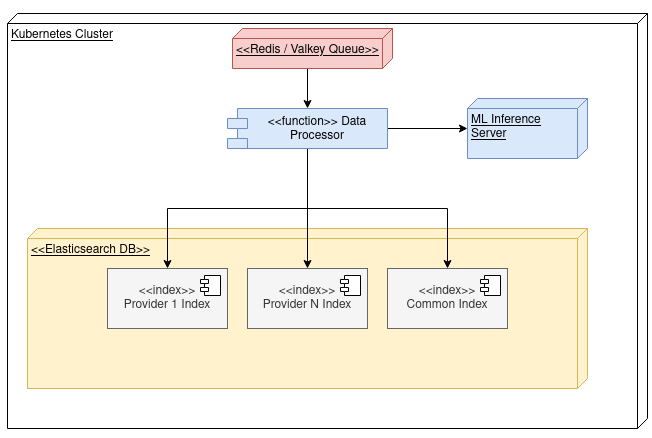
\includegraphics[width=0.5\textwidth]{./assets/DataProcessingArch.png}
        \caption{Data processing pipeline architecture}
        \label{DataProcessingArchitectureFig}  
    \end{center}
\end{figure}

The data obtained from the different sources had different schemas and fields, which made querying data from all of them to study a single problem a challenge. For this reason, we created a common index to store the data from these sources under the same schema, as well as storing the raw-data in provider-specific schemas. This allows us to have both the raw data for validation and further source-specific exploration purposes and the processed data for analysis at the cost of using up more storage space.

As our data of interest was mostly text based, we based our processing around text features and manipulation. ElasticSearch offers native full-text indexing and search capabilities, and we also augmented the text with additional features computed using Machine Learning models. These include text embeddings for semantic search to extend searching capabilities beyond full-text search, sentiment analysis, and emotion classification.

\subsection{Machine Learning Inference}
In order to use ML models for the data enrichment mentioned in section \ref{DataProcessingArchitecture}, we used open source models from HuggingFace along with their Transformers library. In particular, we used the following:
\begin{enumerate}
	\item A sentiment analysis model trained on Twitter texts \cite{tweetnlp}.
	
	\item An emotion detection model \cite{tweeteval}. This is a classification model that outputs an array of emotions detected in the text.
\end{enumerate}

Both of these Machine Learning models were trained specifically on social media data, namely twitter, which made them well suited for our use case. While the models have not been updated in some time, they can still be quite useful for NLP tasks in resource-constrained environments such as ours.

In order to deploy these models, we converted them to ONNX format and deployed a standalone service to perform inference, which exposed a simple HTTP API. Using ONNX allows us to keep the image more lightweight, instead of using a full-blown ML framework with training and other capabilities we do not need. These models are pre-packaged into the docker image to avoid the overhead of downloading and possibly converting them on container startup at the cost of having a larger image.

We deployed this as a Kubernetes deployment exposed via a service within the cluster, with the configuration definitions written in a Helm chart. Using a helm chart means we can more easily modify configurations for the service such as the number of replicas and the version of the Docker image we are using. We are currently using a single replica to be mindful of limited cluster resources, but this container can be horizontally scaled by simply adding more replicas, since it is completely stateless. One could also add a Horizontal Pod Autoscaler to the deployment and allow it to scale elastically with usage, but this is currently not enabled.

The reason we decided to deploy this as a standalone service instead of a Fission function is that in principle FaaS functions should be lightweight, and quick to deploy and run. However, using Transformers models that must be loaded into memory can significantly add to the startup time of the service, even with our optimisations, while once they are loaded into memory inference is relatively fast for the chosen models, even without a GPU. Thus, the benefits of deploying this as a standalone persistent service rather than a Fission function outweighed the overhead of managing some additional Kubernetes resources explicitly.

\subsection{Language Processing Limitations}
While the deployed HuggingFace models proved effective for baseline sentiment and emotion detection, mining social media text presents inherent NLP challenges. Social media discourse is heavily reliant on sarcasm, irony, and culturally specific slang (e.g., Australian colloquialisms), which off-the-shelf models frequently misclassify. For instance, a highly sarcastic post criticizing a political leader's decision might be incorrectly tagged as ``positive'' by the sentiment model due to the presence of outwardly positive vocabulary.

\subsection{Common Index Design}
\label{DataProcessingCommonIndexDesign}
In order to allow easier analysis of the data from all sources, we introduced a common data index. While platform-specific raw indices are useful for preserving the original structure of each data source, they are less convenient for downstream tasks such as topic discovery, sentiment analysis, emotion tagging, and dashboarding across multiple social platforms. To address this, we maintain a platform-neutral document schema in \texttt{social-posts-index}, allowing posts from different sources to be accessed by a single query.

The schema design of the common index is intentionally lightweight. Rather than duplicating every nested field from the original source, we store a core set of cross-platform analytical fields. The mapping includes \texttt{platform}, \texttt{record\_type}, \texttt{platform\_post\_id}, \texttt{common\_id}, \texttt{text}, \texttt{created\_at}, \texttt{ingested\_at}, \texttt{source\_url}, and \texttt{source\_meta}. It also includes a \texttt{sentiment} object with positive, neutral, and negative scores, together with a final sentiment label, and a nested \texttt{emotion} array with label-score pairs. Notably, \texttt{source\_meta} is stored as an object with \texttt{enabled: false}, which means that we preserve provenance or extra metadata without indexing every internal subfield. This provides a practical compromise between traceability and query performance.

Architecturally, the common index acts as the normalized analytical layer of the system. The streaming harvesters produce source-tagged queue messages. These messages can then be consumed by a downstream processor that standardizes fields into the common schema and enriches them with sentiment and emotion outputs. This means that the common index is not merely an additional storage location; rather, it is the layer where heterogeneous platform records become comparable. The design also supports deterministic identifiers through \texttt{common\_id} and explicit \texttt{platform\_post\_id} values, both of which are important for deduplication and for tracing a processed document back to its original source record.

From an analytical perspective, the common index enables queries that would be difficult to perform on platform-specific raw schemas alone. Because the common schema consistently exposes post text, timestamps, source platform, and standardized sentiment and emotion outputs, we can more easily perform cross-platform topic exploration, measure changes over time, compare sentiment trajectories by theme, and support a front-end dashboard that does not need to understand each platform's native data structure. In this sense, the common index serves as the bridge between raw collection and usable social analysis.

We implement this common analytical layer in Elasticsearch as \texttt{social-posts-index}, with a compact cross-platform schema that stores normalized post text, temporal metadata, provenance metadata, and sentiment and emotion annotations. This design supports downstream reporting, dashboarding, and comparative analysis across multiple social sources while still retaining enough metadata to trace results back to platform-specific records when necessary. 


\subsection{Error Handling and Safeguards}
We added some error handling mechanisms to the processor in order to avoid some potential pitfalls or failure modes. Two that we considered pressing were:
\begin{itemize}
	\item Errors in MQTTrigger or in the processing function. We added an error queue to the MQT Trigger configuration for Fission to catch these error messages. These arose either when the processing function threw an exception for some reason, or when the trigger failed to call an available processor function (see \ref{TechnicalDiscussion}). These errors could then be re-inserted into the processing queue for another try, or un further inspection discarded. This could be done automatically, and one could add a retry limit, but for our case we audited these errors manually.
	
	\item Duplicate inserts. This could arise, for example, if a streaming function spun up before the prevous one had exited. In order to handle such cases, we use Valkey to keep a cache of the IDs of records we have inserted in the last 2 hours to avoid duplicate inserts of fresh data. For historical data, deduplication can be handled in other ways, such as by querying the database directly to see which IDs already exist, but in the real-time processing scenario, caching is a quicker and cheaper alternative to this.
\end{itemize}
